% ****** Start of file aipsamp.tex ******
%
%   This file is part of the AIP files in the AIP distribution for REVTeX 4.
%   Version 4.1 of REVTeX, October 2009
%
%   Copyright (c) 2009 American Institute of Physics.
%
%   See the AIP README file for restrictions and more information.
%
% TeX'ing this file requires that you have AMS-LaTeX 2.0 installed
% as well as the rest of the prerequisites for REVTeX 4.1
%
% It also requires running BibTeX. The commands are as follows:
%
%  1)  latex  aipsamp
%  2)  bibtex aipsamp
%  3)  latex  aipsamp
%  4)  latex  aipsamp
%
% Use this file as a source of example code for your aip document.
% Use the file aiptemplate.tex as a template for your document.
\documentclass[
aip,
%jmp,%
%bmf,%
%sd,%
rsi,%
amsmath,amssymb,
%preprint,%
reprint,%
%author-year,%
%author-numerical,%
]{revtex4-1}

\usepackage{graphicx}% Include figure files
\usepackage{dcolumn}% Align table columns on decimal point
\usepackage{bm}% bold math
%\usepackage[mathlines]{lineno}% Enable numbering of text and display math
%\linenumbers\relax % Commence numbering lines

\newcommand	 {\sbar}	{{s}}
\newcommand	 {\rbar}	{{r}}
\newcommand	 {\hi}		{{h_\mathrm{i}}}
\newcommand	 {\pii}  	{{p_\mathrm{i}}}
\newcommand	 {\kb}		{{k_\mathrm{B}}}
\newcommand	 {\Tlow}	{{T_\mathrm{low}}}
\newcommand 	 {\Pnat} 	{{P_\mathrm{nat}}}
\newcommand {\QIA}	{{Q_\mathrm{IA}}}
\newcommand {\QIB}	{{Q_\mathrm{IB}}}
\newcommand {\QIIA}	{{Q_\mathrm{IIA}}}
\newcommand {\QIIB}	{{Q_\mathrm{IIB}}}
\newcommand {\Pcut}     	{{P_\mathrm{cut}}}
\newcommand {\TlowI}     {{T^\mathrm{I}_\mathrm{low}}}
\newcommand {\TlowII}    {{T^\mathrm{II}_\mathrm{low}}}
\newcommand {\Ptot}	{{P_\mathrm{tot}}}
\newcommand {\PIA}    	{{P_\mathrm{IA}}}
\newcommand {\PIB}    	{{P_\mathrm{IB}}}
\newcommand {\PIIA}    	{{P_\mathrm{IIA}}}
\newcommand {\PIIB}    	{{P_\mathrm{IIB}}}
\newcommand {\Eave}	{{E_\mathrm{ave}}}
\newcommand {\sigE}	{{\sigma_{\left < E \right >}}}
\newcommand {\SR}		{${\mathrm{S16}_{144}}$}
\newcommand {\SI}		{${\mathrm{S16}_{1024}}$}	
\newcommand {\SII}		{${\mathrm{S35}_{1024}}$}

\begin{document}

\preprint{AIP/123-QED}

\title[Multisequence Monte Carlo simulations]{Multisequence algorithm for coarse-grained biomolecular simulations: application to protein fold switching}

\author{A. Aina}
\author{S. Wallin}
\email{swallin@mun.ca}
\affiliation{ 
Memorial University of Newfoundland, Department of Physics and Physical Oceanography, A1B 3X7 St John's, NL, Canada}

\date{\today}

\begin{abstract}
We consider a generalized-ensemble algorithm for coarse-grained simulations of biomolecules which allows the thermodynamic behavior of two or more sequences to be determined in a single ``multisequence" run. By carrying out a random walk in sequence space, the method also enhances conformational sampling. Escape from local energy minima is accelerated by visiting sequences for which the minima are more shallow or absent. We apply the method alongside an intermediate-resolution coarse-grained model for protein folding with 7 atoms per amino acid and 3 amino acid types. The potential for large-scale coverage of sequence space is explored by applying the method to two sets with $>$1,000 sequences each. The resulting thermodynamic data is used to explore the sequence-structure and sequence-stability relationships between pairs of protein folds with different secondary structures.
\end{abstract}

\pacs{87.14.E; 87.15.A; 05.10.Ln}
                             
\keywords{Monte Carlo, generalized ensembles, simulated tempering, protein folding, protein evolution}

\maketitle

\section{Introduction}
\noindent
Recent years have seen important advances in biomolecular simulation methods, including improvements to standard molecular dynamics force fields,~\cite{Piana2014} the advent of several alternative atomistic simulation approaches,~\cite{Ding2008,Irback2006,Verma2009,Yang2007} and new techniques for  conformational sampling.~\cite{Bernardi2015} These advances have in part triggered major efforts~\cite{McGuffee2010,Perilla2016,Lindorff-Larsen2011,Yu2016} to characterize the molecular dynamics of bio-systems of different sizes, e.g., a small native protein on the millisecond scale~\cite{Lindorff-Larsen2011} or a comprehensive model cytoplasm on the nanosecond scale.~\cite{Yu2016} While encouraging and insightful, these large-scale simulations have also highlighted the fact that severe tradeoffs in size and time scales will likely persist for the foreseeable future for detailed simulations. 

One way to expand the range of biomolecular simulations is to turn to coarse-grained (CG) models, where the basic aim is to simplify the physical description of interactions while retaining the essential physics of the system under study.~\cite{Riniker2012} Ingolfsson \textit{et al.} list 4 main factors that make CG models computationally fast: reduction in the number of degrees of freedom, faster simulation dynamics, emphasis on short-range interactions and the ability of using larger integration time steps.~\cite{Ingolfsson2014} To this list can be added that a CG representation either of the interaction potential or the molecular geometry often opens up for alternative sampling schemes beyond traditional molecular dynamics approaches which can further speed up conformational sampling, e.g., activation-relaxation kinetics,~\cite{Beland2011} discrete molecular dynamics~\cite{Proctor2011} and various Monte Carlo (MC)-based techniques such as cluster moves.~\cite{Vitalis2009} 

The challenges of achieving representative conformational sampling of individual biomolecular systems notwithstanding, a range of systems naturally call for the investigation and comparison of many molecular variants, e.g., determining the molecular mechanisms of specificity in protein-protein~\cite{Zarrinpar2003,Hakes2007} or protein-nucleotide interactions,~\cite{Rohs2010} or the role of mutations in disease processes such as protein aggregation.~\cite{Ross2004} Another example is protein folding where unique insight has been achieved by comparing the folding within and between protein families.~\cite{Tzul2017,Wensley2010} With the increasing availability of sequence information,~\cite{Vukmirovic2000} it is of interest to explore ways to efficiently sample multiple sequences in biomolecular simulations. 

To this end, we evaluate in this work an MC-based algorithm that can in principle calculate the thermodynamics of multiple sequences in a single run and apply it to a coarse-grained model for protein folding. This ``multisequence" (MS) method was originally developed in the context of homo- and heteropolymer simulations~\cite{Irback1995} and was later adapted for the characterization of peptide-protein binding specificity,~\cite{Bhattacherjee2013,Wallin2017}, but it has to our knowledge not been previously tested in protein folding simulations. The MS algorithm relies on sampling at fixed temperature a generalized ensemble in which the sequence is a dynamic parameter. Hence, there are two main types of updates: conformational updates $\rbar\rightarrow\rbar'$ and sequence updates $\sbar\rightarrow\sbar'$. As illustrated in Fig.~1, this approach is easily applied when $\rbar$ and $\sbar$ are ``perpendicular" coordinates such that the potential energy of the model can be written in terms of two independent variables, $E(\sbar,\rbar)$. While this may be hard to achieve for detailed protein models, it is likely possible in many CG models.

As an initial test case, we apply the MS method to a set of 144 model sequences with 16 amino acids. This set, {\SR}, was constructed to sparsely cover the sequence space between two ideally designed sequences, A1 and N1, which fold into an $\alpha$-helix and $\beta$-hairpin, respectively, and allowed us to demonstrate the existence of A1-N1 mutational pathways which abruptly switch between the two structures and do not proceed through unstable sequences.~\cite{Holzgrafe2014} Here we use this set to validate the MS method and compare its efficiency to a standard generalized-ensemble method, namely simulated tempering (ST).~\cite{Marinari1992,Lyubartsev1992} We thereafter apply the MS method to a greatly enlarged set with 1,024 sequences, also spanning the A1-N1 space, as well as another set spanning two 35-amino acid sequences, A2 and TN, that fold into two-helical bundle and mixed $\alpha$-$\beta$ structures, respectively. Besides hinting at the feasibility of applying the MS method on large sets of sequences, the results allow us to carry out a more systematic analysis of the biophysical properties of sequences along mutational pathways connecting these two pairs of basic protein folds than has been possible with standard methods.~\cite{Holzgrafe2014,Holzgrafe2015} 

%We find that sequences become gradually less stable as they approach switch point. However, fold switching is observed to be typically abrupt at the switch point. Folding pathways usually pass through bistable sequences which populate both folds up to a significant level. We show that while bistable sequences become less when selecting more stable pathways for A1-N1 system, they generally remain the same for the A2-TN system.


%We first apply the MS algorithm to a set of 144 model sequences with 16 amino acids and compare with the simulated tempering (ST) algorithm. We find that the computational efficiency of the MS algorithm is never less than ST except at the lowest studied temperature for one sequence. 



%We then demonstrate that the multisequence algorithm can be used to calculate the thermodynamic behavior for $>1,000$ sequences in a 3-letter model for protein folding~\cite{Bhattacherjee2012} at temperatures well below the typical folding temperatures $T_\mathrm{f}$ of the included sequences.  

%Modern investigations into biophysical properties of biomolecular systems are routinely carried out not only on a single species but on multiple molecular variants.~\cite{Vukmirovic2000,Nickson2010} For example, protein engineering methods are used to provide mechanistic insight into the specificity of protein-protein and protein-DNA interactions, to compare the  conformational propensities of disease-related mutations of aggregation-prone proteins, and optimize biomolecular properties through directed evolution. Moreover, large-scale screening techniques such as phage display and microarray chips are used to provide biophysical properties across entire genomes. In short, through the study of a biomolecular system and related variants molecular variants are studied in order to gain a more complete picture of the biophysical and biochemical properties of the system and provide evolutionary context. 

%While protein or DNA sequences are easily changed on the computer, the high computational cost of simulating even a single moderately-sized biomolecule makes systematic explorations of sequence space challenging. Some notable efforts have nonetheless been attempted, including simulations of all 136 unique tetranucleotide sequences in B-DNA oligonucleotides using all-atom explicit water molecular dynamics.~\cite{Beveridge2004}



%While the 16-amino acid A1 and N1 sequences fold into $\alpha$-helical and $\beta$-hairpin folds, respectively, the two 35-amino acid sequences A2 and TN adopt the folds denoted IIA and IIB, as shown in Fig.~X. 



\begin{figure}
\includegraphics[width=4.2cm]{Fig1}
\caption{The two types of Monte Carlo updates in the multisequence Monte Carlo algorithm.}
\end{figure}

\section{Theory}

\subsection{Generalized-ensemble algorithms and simulated tempering}
\noindent
Conventional Monte Carlo simulations of the canonical distribution is problematic at low temperatures $T$ for many physical systems because simulations tend to become trapped in local energy minima and hamper representative sampling of configurational space. The basic idea of generalized-ensemble algorithms~\cite{Mitsutake2001} is to alleviate this trapping problem by sampling states using a non-Boltzmann weight factor and/or expand the state space with additional dynamical parameters, such that a more efficient random walk in potential energy can be achieved. 

A well-known generalized-ensemble algorithm is simulated tempering (ST),~\cite{Marinari1992,Lyubartsev1992} in which it is the temperature $T$ that becomes a dynamic parameter. In this scheme, frequent visits to high-$T$ allow simulations to readily escape from local energy traps. The ST algorithm thus simulates the joint probability distribution 
\begin{equation}
P(\rbar,m) =\dfrac{1}{\hat{Z}} e^{-\beta_m E(\rbar) + g_m}\,,
\label{ST}
\end{equation}
where  $\beta_m=1/k_\mathrm{B} T_m$, $\{T_m\}_{m=1}^\mathrm{M}$ a set of temperatures and $k_\mathrm{B}$ is Boltzmann's constant. The normalization constant in Eq.~\ref{ST} is  
\begin{equation}
\hat{Z} = \sum_r \sum_{m=1}^{\mathrm{M}}e^{-\beta_m E(\rbar) + g_m}\,,
\end{equation}
where the first sum is over all conformations $\rbar$. The simulation parameters $g_m$ control the marginal probability distribution
\begin{equation}
P(m) = \frac{1}{\hat{Z}}\sum_r e^{-\beta_m E(\rbar) + g_m} \,,
\end{equation}
and must therefore be carefully chosen. A common and convenient choice is $g_m\approx \beta_m F_m$, where $F_m$ is the free energy at temperature $T_m$. With this choice, $P(m)$ becomes approximately flat ensuring all temperatures are frequently visited. 

\subsection{Multisequence algorithm}
\noindent 
The basic idea of the MS algorithm for biomolecular simulation is to let the sequence $\sbar$ become a dynamic parameter rather than the temperature as in ST. A dynamic $\sbar$ is technically feasible as long as the potential energy can be written as $E(\sbar,\rbar)$, where $\sbar$ and $\rbar$ are independent variables. This is the case in our coarse-grained protein model with only backbone degrees of freedom and can also be achieved for more detailed  models~\cite{Bhattacherjee2013,Wallin2017}. 

In analogy with ST, the MS algorithm simulates the joint probability distribution
\begin{equation}
P(\sbar,\rbar) =\dfrac{1}{\tilde{Z}}e^{-\beta E(\sbar,\rbar) + h(\sbar)}\,, 
\label{MS}
\end{equation}
where  
\begin{equation}
\tilde{Z} = \sum_{\sbar}\sum_{\rbar} e^{-\beta E(\sbar,\rbar)+ h(\sbar)}\,
\end{equation}
and the first sum goes over a set of allowed sequences $\sbar$. The simulation parameters $h(\sbar)$, similar to the parameters $g_m$ in ST, control the marginal distribution $P(\sbar)=\tilde{Z}^{-1}\sum_{\rbar} e^{-\beta E(\sbar,\rbar)+ h(\sbar)} = \tilde{Z}^{-1}e^{-\beta F(\sbar)+ h(\sbar)}$ and a roughly flat $P(\sbar)$ can be achieved by choosing $h(\sbar) \approx \beta F(\sbar)$, where $F(\sbar)$ is the free energy of sequence $\sbar$ at temperature $T$. 

Two types of MC updates are required to sample from the distrubution in Eq.~\ref{MS}, ordinary conformational update $\rbar\rightarrow\rbar'$ and mutational updates $\sbar\rightarrow\sbar'$. The acceptance probabilities for the latter  becomes
\begin{equation}
P_\mathrm{acc} (\sbar\rightarrow\sbar') = \min [1, \exp\{-\beta\Delta E+\Delta h\}]\,,
\label{accrej}
\end{equation}
where $\Delta E = E(\sbar',\rbar)-E(\sbar,\rbar)$ and $\Delta h = h({\sbar'})-h(\sbar)$.

\section{Model and Methods}
\subsection{Coarse-grained 3-letter model for protein folding}
\noindent
All calculations were carried out using the coarse-grained model for protein folding developed in Ref.~\citenum{Bhattacherjee2012}. In this model, there are 3 different amino acid types: hydrophobic (h), polar (p) and turn-type (t). The backbone chain is represented atomistically by the N, H, $\mathrm{C}_\alpha$, $\mathrm{H}_{\alpha 1}$, C$'$ and O atoms. By contrast, the sidechain represention is simplified to a single enlarged $\mathrm{C}_\beta$ atom, which is geometrically identical for h and p types. The sidechain is absent for the t type which instead has an $\mathrm{H}_{\alpha 2}$ atom. The t type is therefore closely related to glycine. All bond lengths, bond angles, and peptide plane angles (180$^\circ$) are held fixed. Hence, an $N$-amino acid chain conformation $\rbar$ can, for any sequence $\sbar$, therefore be described by the set of 2$N$ backbone torsional angles $\{\phi_i$, $\psi_i\}_{i=1}^{N}$. 
 
This geometrical description is paired with a simplified but finely tuned energy function with 4 terms: $E= E_\mathrm{ev} + E_\mathrm{loc} + E_\mathrm{hb} + E_\mathrm{hp}$. The first two, $E_\mathrm{ev}$ and $E_\mathrm{loc}$, represent excluded-volume effects of all atoms and local electrostatic effects, respectively. The hydrogen-bond energy, $E_\mathrm{hb}$, represents directionally dependent interactions between NH and CO groups which are necessary for secondary structure formation. Finally, the ``hydrophobicity" term, $E_\mathrm{hp}$, implements pairwise Lennard-Jones-like interactions between the $C_\beta$ atoms of h amino acids which are necessary for driving chain collapse during folding. Various model parameters, e.g., the strengths of hydrophobic attractions and hydrogen bonding, were determined based on the ability of the model to spontaneously fold a set of model sequences with 18-54 amino acids into  structurally diverse and thermodynamically stable native states with both $\beta$ and $\alpha$-structure. As it turned out, this strategy made the model robust enough to fold sequences designed to have mixed $\alpha$ and $\beta$ structures. 

\subsection{Model sequences}
\noindent
Six of the model sequences studied in this work, A1, N1, R1, R2, A2, and TN, are given in Table~I. In addition, we study two sequence sets $\mathrm{S16}_{1024}$  and $\mathrm{S35}_{1024}$ with 1,024 sequences each derived from the A1-N1 and A2-TN pairs, respectively, through mutational combinations, as well as the set $\mathrm{S16}_{144}$ taken from  Ref.~\protect\citenum{Holzgrafe2014}. 
 
\begin{table}
\caption{\label{tab1} List of 6 model sequences of different lengths $N$ studied in this work.}
\begin{ruledtabular}
\begin{tabular}{lcr}
Name & $N$ & Sequence \\
\hline
A1 & 16 & pphpphhpphpphhpp \\
N1 & 16 & phphphpttphphphp \\
R1 & 16 & pphhphptthpphhpp\\
R2 & 16 & ppphphhtthhphppp\\
A2 & 35 & (A1)ttt(A1)\\
TN & 35 & (A1)ttt(N1)\\
\end{tabular}
\end{ruledtabular}
\end{table}


\subsection{Monte Carlo simulation parameters}
\noindent
Both ST and MS simulations are carried out with two types of conformational updates $\rbar\rightarrow\rbar'$: (1) a global pivot move (20\%) which randomly picks a $\phi_\mathrm{i}$ angle or $\psi_\mathrm{i}$ angle and assign a new value between $-\pi$ and $\pi$; and (2) a semi-local move (80\%) which turns the $\phi_\mathrm{i}$ and $\psi_\mathrm{i}$-angles of 4 consecutive amino acids in a coordinated manner.~\cite{Favrin2001} In MS simulations, sequence updates $\sbar\rightarrow\sbar'$ are carried out by randomly picking a new sequence $\sbar'\ne\sbar$ and applying the accept-reject criterion in Eq.~\ref{accrej}. A sequence move is attempted every $1,000$ MC steps while temperature updates $m\rightarrow m'$ are attempted every 100 steps. The simulations carried out in this work are summarized in Table~II.

\begin{table}
\caption{\label{tab2} List of simulations carried out in this work. }
\begin{ruledtabular}
\begin{tabular}{lcccr}
Runs & Algorithm & $\kb T$  & MC steps/run\footnote{Excludes a thermalization step with $10^6$ MC steps/run.} &  Sequences\\
\hline
32 & ST & 0.43--0.65 & $1\times10^7$ &A1\\ 
32 & ST & 0.43--0.65 & $1\times10^7$ &N1\\ 
32 & ST & 0.43--0.65 & $1\times10^7$ &R1\\ 
32 & ST & 0.43--0.65 & $1\times10^7$ &R2\\ 
32$\times$8\footnote{32 runs per temperature at 8 different temperatures.} & MS &0.43--0.65& $18\times 10^7$ & $\mathrm{S16}_{144}$\\
16 & MS & 0.43  & $5\times 10^9$ &  $\mathrm{S16}_{1024}$ \\
16 & MS & 0.46 & $4\times 10^9$ &  $\mathrm{S35}_{1024}$ \\
\end{tabular}
\end{ruledtabular}
\end{table}

\subsection{Observables}
\noindent
Fold stabilities are calculated as in Ref.~\citenum{Holzgrafe2015} and described briefly below. First we define two structural similarity measures $\QIA$ and $\QIB$ for folds IA and IB, respectively, indicating the fraction of the fold-specific backbone-backbone hydrogen bonds that have been formed. The fold IA-hydrogen bonds are (2,6), (3,7), (4,8), (5,9), (6,10), (7,11), (8,12), (9,13), (10,14), (11,15) and the fold IB-bonds are (3,14), (5,12), (7,10), (10,7), (12,5), (14,3), where (i,j) indicates a hydrogen bond between the CO group of amino acid i and the NH group of amino acid j. The  stabilities of folds IA and IB are then defined as the probabilities $\PIA = P(\QIA\ge0.8)$ and $\PIB = P(\QIB\ge0.80)$, respectively, i.e., the probability that at least 80\% of the fold's hydrogen bonds are formed. $\PIA$ and $\PIB$ thus depend on both sequence $\sbar$ and temperature $T$. For example, $\PIA=0.875\pm 0.003$ for A1 and $\PIB=0.785\pm0.008$ for N1 at $\kb T = 0.43$. Structural similarity measures for 35-amino acid folds IIA and IIB are defined as $\QIIA = ( Q_\mathrm{IA}^\mathrm{1-16} + Q_\mathrm{IA}^\mathrm{20-35} + Q_\mathrm{tert} ) / 3$ and $\QIIB = ( Q_\mathrm{IA}^\mathrm{1-16} + Q_\mathrm{IB}^\mathrm{20-35} + Q_\mathrm{tert} ) / 3$, respectively, where superscripts on $\QIA$ and $\QIB$ indicate over which amino acid positions those measures are applied to within the longer 35 amino acid sequences and $Q_\mathrm{tert}$ is a measure that counts the number of $\mathrm{C}_\beta$-$\mathrm{C}_\beta$ contacts between the two secondary structure elements of these folds.~\cite{Holzgrafe2015} In analogy with $\PIA$ and $\PIB$, we define the stabilities of folds IIA and IIB as $\PIIA = P(\QIIA\ge0.8)$ and $\PIIB = P(\QIIB\ge0.80)$, respectively. The root-mean-square-deviation, RMSD, is calculated over all $\mathrm{C}_\alpha$ atoms.

\begin{figure}
\includegraphics[width=10.0cm]{MCTrajFolds}
\caption{(A) Example of an MS simulation applied to the sequence set $\mathrm{S16}_{144}$. The plot shows the MC evolution of the sequence $\sbar$ (numbered 1--144), the total potential energy $E$ and the root-mean-square deviation (RMSD) calculated against fold IA (light blue) and fold IB (dark red) structures shown in (B). The simulation is carried out at $\kb T = 0.43$. (B) Representative structures of fold IA and fold IB, selected to be the minimum-energy conformations found for the sequences A1 and N1, respectively. (C) Representative fold IIA and fold IIB structures selected to be the minimum-energy conformations of A2 and TN, respectively. }
\end{figure}

\section{Results}

\subsection{Computational efficiency of the multisequence algorithm}
\noindent
We start by testing the MS algorithm on the set {\SR} consisting of the 144 3-letter model sequences with 16 amino acids studied in Ref.~\citenum{Holzgrafe2014}. Two of the sequences in {\SR} are A1 and N1 (see Table~I) which were designed to fold into stable $\alpha$-helix and $\beta$-hairpin structures, respectively, as shown in Fig.~2B. A1 and N1 differ at 10 positions such that 10 consecutive point mutations can transform A1 into N1, and vice versa. The binary sequence space between A1 and N1 in which any combination of these mutations have been carried out, therefore contains $2^{10}=1,024$ sequences. The 144 sequences were selected from this binary space with the constraint that the total number of h-amino acids are not too high and not too unevenly distributed.~\cite{Holzgrafe2014}

\begin{figure}
\includegraphics[width=7.8cm]{Pacc}
\caption{Acceptance rates for $\sbar\rightarrow\sbar'$ updates in MS simulations of the {\SR} sequence set as a function of (A) the number of changed amino acid positions $\Delta h$ and (B) temperature $T$. Acceptance rates for 3 different $T$'s are shown in (A).}
\end{figure}

We apply the multisequence algorithm on the set {\SR} across a range of temperatures (see Table~II). Figure~2 illustrates a typical MS simulation trajectory carried out at the lowest temperature which is well below the folding temperature of both A1 and N1~\cite{Holzgrafe2014,Holzgrafe2015}. From the MC evolution of the total energy $E$, sequence index $\sbar$, and RMSD values from the representative structures in Fig.~2B, it is evident that visits to various sequences drive transitions into a range of structural states. In particular, there are frequent visits to both $\alpha$-helix and $\beta$-hairpin structures. Transitions between them are accompanied by a shift in which sequences are preferably visited. For example, visits to high $\sbar$-indices, including N1 with index 144, tend to coincide with formation of $\beta$-hairpin structures.

One might have suspected that the MS algorithm would be hampered by poor acceptance rates for sequence updates. However, this is not the case. We carry out updates $\sbar\rightarrow\sbar'$ by picking a new random sequence $\sbar'\ne\sbar$ from the set of allowed sequences. The (average) acceptance rate  depends on both $T$ and the step in sequences space $\Delta h$, i.e., the number of amino acid positions changed, as shown in Fig.~3. At the lowest $T$ and high $\Delta h$, acceptance rates are only around 0.1-0.2 but are substantially higher at other $T$ and $\Delta h$ values. The overall acceptance rates are in fact above the oft-quoted rule-of-thumb value $0.25$~\cite{Gilks1996} for all temperatures $T$ (see Fig~4B). Increased acceptance rates can easily be achieved by restricting proposed updates such that $\Delta h\le\Delta h_\mathrm{max}$, where $\Delta h_\mathrm{max}$ is a maximum step size, which might be necessary for longer protein chains. 

\begin{figure}
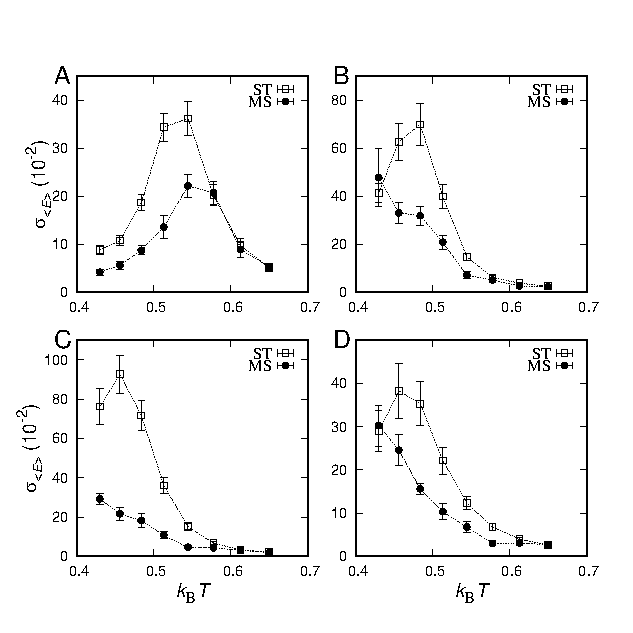
\includegraphics[width=8.0cm]{Stderr}
\caption{Comparing sampling efficiency of the MS and ST algorithms. Statistical errors $\sigma_{\left < E\right >}$ of the average total energy $\left < E\right >$ from the two methods for the 16-amino acid sequences (A) A1, (B) N1, (C) R1 and (D) R2. Simulation lengths in the two methods are adjusted such that the number of conformations sampled per sequence and temperature is roughly the same (see text). }
\end{figure}

We now compare the results from our MS calculations with simulated tempering (ST) simulations carried out on 4 of the 144 sequences, namely A1 and N1 and two sequences, R1 and R2, chosen randomly at distances $h=4$ and $h=6$ from A1, respectively (see Table~I). While ST provides the thermodynamics of a given sequence across a range of $T$ in a single run, a MS simulation provides the thermodynamics of all 144 sequences for one $T$. We adjust the simulation lengths for ST and MS runs such that roughly the same number of sampled conformations are obtained for each $\sbar$ and $T$ combination, thus ensuring that similar computational resources are used for the two algorithms (see Table~II). The MS algorithm is validated by comparing the average total energy, $\left < E \right >$, calculated for different $T$'s and $\sbar$'s, between the two sets of results (see Supplementary Information). 

As a way to assess sampling efficiency, we compare in Figure~4 the statistical error, $\sigE$, of the average energy $\left <E\right >$ for the 4 different sequences obtained using ST and MS, respectively. Since roughly the same number of sampled conformations were obtained for each $\sbar$ and $T$ combination, we compare the statistical errors directly. The two algorithms give similar errors at the highest $T$ studied which implies consistent result between them. It should be noted that the highest $T$ studied is well above the folding temperature for all the 4 sequences. Therefore, this consistency is not particularly surprising since at high-T the free-energy landscape is relatively smooth. Hence, conformational space requires little difficulty to sample.

However, as temperature decreases, the statistical error from the MS algorithm generally becomes smaller than those from ST. In particular, Fig.~4C illustrates that MS is on average twice as accurate as ST in its error estimates for R1. The best estimate occurs at $\kb\approx$ 0.46 where MS is about 450\% better than ST. Even at the lowest T studied, MS is at least consistent or better than ST for all 4 sequences.


\begin{figure*}
\rotatebox{0}{\includegraphics[width=16.6cm]{network}}
\caption{Networks of sequences connecting folds IA and IB (top) and folds IIA and IIB (bottom). Each node represents a stable sequence ($\Ptot\ge\Pcut$ where $\Pcut=0.50$) that folds into either IA or IIA (light blue), IB or IIB (dark red), or is classified as bistable ($B>0.5$, black). A line between two nodes indicates that the sequences differ at only one position. Graph created using the tool Graphviz~\protect\cite{Graphviz2000} obtained from  www.graphviz.org.}
\end{figure*}

%Hence, we conclude that in the comparison made above the computational efficiency of the MS algorithm is comparable to ST. It must be stressed, however, that while the ST simulation requires that the thermodynamic behavior is calculated at a range of temperatures, MS works well on its own directly at low temperatures. ST was introduced as an extension to the standard, fixed-$T$ Metropolis-Hastings algorithm in order to overcome the poor mixing of states at low temperatures, i.e., the tendency for the simulations at low $T$ to become trapped in local free energy minima. The MS algorithm, however, efficiently calculates the thermodynamics at low $T$'s without visits to other $T$'s. In the MS algorithm, it is visits to sequences with poor native state stability rather than high $T$'s that drive the decorrelation of generated states and escape from local traps. This way, calculation of low-$T$ thermodynamics is enhanced in MS simulations while at the same time enhancing coverage in sequence space. This makes the MS algorithm ideal for situations in which the finite-$T$ thermodynamic behavior of multiple sequences are of interest. 

\vspace{12pt}
\subsection{A1-N1 and A2-TN binary sequence space}
\noindent
We now turn to the full binary sequence sets {\SI} and {\SII} with 1,024 sequences each. By applying the MS method to these two sets separately (see Table~II), we determined the thermodynamic behavior of each included sequence at relatively low temperatures. In particular, these simulations allowed us to find the stabilities relative to folds IA and IB ($\PIA$ and $\PIB$) for all sequences in {\SI} and the stabilities relative to folds IIA and IIB ($\PIIA$ and $\PIIB$) for all sequences in {\SII}.

Having calculated these fold stabilities, we are in a position to determine if there are pathways in sequence space that lead to IA-IB or IIA-IIB fold changes without passing through an unstable intermediate sequence. To this end, we construct graphs in which each stable sequence is represented by a node and any two nodes are connected if their sequences differ at only one amino acid position. To determine if a sequence is stable we used the criterion $P_\mathrm{tot}>\Pcut$, where  $\Ptot = \PIA + \PIB$ and $\PIIA + \PIIB$ for A1-N1 and A2-TN, respectively. The precise network obtained depends, of course, on the cut-off value of $\Pcut$. In general, a higher $\Pcut$ means a selection of more stable pathways. Fig.~5 shows the networks obtained with $\Pcut=0.50$. The number of viable mutational pathways that connect the start and end points are 516,972 between A1 and N1 and  57,912 between A2 and TN. Because there are $10! =3,628,800$ possible mutational pathways between start and end points in both cases, these pathways represent 14.2 \% and 1.6 \% of all possible pathways in A1-N1 and A2-TN, respectively. Hence, A1 and N1 are rather highly connected at this stability threshold. For $\Pcut=0.60$, the numbers are 104,640 pathways (2.9\%) for A1-N1 and 22,512 (0.6\%) pathways for A2-TN. We find that there are no possible A1-to-N1 or A2-to-TN pathways when $\Pcut\ge0.74$ and $\Pcut\ge 0.66$, respectively. \\

\subsection{Stability and bistability properties in of fold-to-fold mutational pathways}
\noindent 
An apparently general characteristic of designed and natural protein folding switching is that sequences near the switch point have reduced stability.~\cite{Bryan2010} The results from our model exhibit a similar trend. Fig.~6A and B show the total stability $\Ptot$ at different mutational distances between start and end points. Intermediate sequences are less stable than sequences at distances $h=0$ and $h=10$, although there are large variations as indicated by the spread between upper and lower bounds. Nonetheless, there is a clear statistical trend that sequences become gradually less stable as successive mutations are applied to any of the 4 start and end points until a minimum is reached. 
%These minima in stability occur closer to N1 and TN in the two systems, respectively, indicating that the IA/IIA folds are more mutationally robust than the IB/IIB folds. 

\begin{figure}
\includegraphics[width=7.8cm]{Paths}
\caption{Stability properties of mutational pathways. The total stability $\Ptot$ as a function of the distance $h$ from A1 averaged over all (A) IA-IB and (B) IIA-IIB mutational paths obtained with $\Pcut=0.50$. Error bars indicate maximum and minimum $\Ptot$ values. The distribution of switch lengths $L_\mathrm{s}$ for the (C) IA-IB and (D) IIA-IIB mutational paths ($\Pcut=0.50$). C and D insets: Average switch length $\left < L_\mathrm{s}\right >$ across all paths as a function of $\Pcut$. Scatter plots of $\Ptot$ versus bistability $B$ for all sequences in (E) {\SI} and (F) {\SII}, where $B=1-\Delta P/\Ptot$ and $\Delta P = |\PIA-\PIB|$ or $|\PIIA-\PIIB|$.}
\end{figure}

%The smooth average stability trends in Fig.~6 might have been underpinned by individual mutational pathways that gradually shift the population between the two folds, however, this is not the case.

However, the smooth stability trends in Fig.~6A and B belie the real character of the individual mutational pathways which tend to exhibit an abrupt switch between the two folds. To examine the statistics of fold transitions in our model, we first make a distinction between two types of stable sequences: those that fold into a single unique fold, thus behaving as classical proteins, and those that exhibit significant stabilities of both folds. Such ``bistable" sequences are interesting from a biophysical perspective in that they alternate between populating two different folds and hence are highly dynamic proteins. Indeed, they have been proposed to play an important role in the evolution of new protein folds.~\cite{Sikosek2016} 

We consider a stable sequence to be bistable if $B>0.5$, where $B$ is a bistability measure (see Fig.~6 legend). In principle, a fold transition can occur directly between two classical proteins with unique folds, or it can proceed via one or more intermediate bistable sequences which populate both folds. We  define the switch length of a mutational pathway $L_\mathrm{s}=2+n_\mathrm{B}$, where $n_\mathrm{B}$ is the number of bistable sequences in between the two classical sequences that define the switch point. Hence, a path with $L_\mathrm{s}=2$ accomplishes a fold switch in a single mutational step without going through a bistable point. From the distributions of  $L_\mathrm{s}$ in Fig.~5C and D taken over all pathways with $\Pcut=0.50$, it can be seen that fold switching along individual pathways are typically completed in only 1-2 mutations and often a single step is enough switch between the IA and IB folds. Hence, fold switching is typically abrupt and, for $\Pcut = 0.5$, it is fairly common that viable pathways pass through one or two bistable sequences. 

Interestingly, IA-IB fold switching through one or more bistable sequences become less and less common as selections for more stable pathways are made. This can be seen from the decrease in $\left <L_\mathrm{s}\right >$ as a function of $\Pcut$ (see Fig.~5C(inset)). For $\Pcut\ge0.70$, there are no longer any viable pathways between the $\alpha$-helix and $\beta$-hairpin that passes through a bistable sequence because $\left <L_\mathrm{s}\right > =  2$. An underlying reason for the occurrence of sharper fold switches for more stable mutational pathways is apparent from a comparison between $\Ptot$ and $B$ across all sequences in {\SI}. As shown in Fig.~5E, sequences with the highest $\Ptot$ tend to exhibit very little bistability. Hence, highly stable mutational pathways are therefore forced to go through abrupt switch points, thereby transitioning between folds in a single mutational step. The situation for the IIA-IIB fold switch is more complicated. Sequences in {\SII} too follow the trend that high overall stability is achieved for only classical proteins with a single dominant fold. However, bistable sequences nonetheless play a crucial role in bridging the IIA-IIB folds because paths without bistable intermediate sequence are not available for $\Pcut\ge0.50$.  Hence, passing through sequences with bistable properties may still be required to achieve mutation-induced fold switching between certain fold pairs even through it lead to a reduced stability at the switch point. 
 
%The sequences {\SII} do also follow this same trend (Fig.~5F). However, bistable sequences do play a crucial role in bridging the folds IIA and IIB even though their stabilities are significantly reduced, all stable mutational pathways must pass through one bistable sequences. \\

%\subsection{Super-highways in sequence space}
%
%While there are a large number possible pathways (for $\Pcut<0.60$) in both systems, there are relatively few ways to pass between the two neutral nets. For $\Pcut=0.50$, we find that there are 109 nodes in the IA neutral net and 34 nodes in the IIB neutral net through which all viable pathways pass. For $\Pcut=0.60$, these numbers reduce to 14 and 10 nodes in the IA and IIA neutral nets, respectively.
%
 
\section{Discussion}
\noindent
The simulation algorithm for biomolecules considered here works by making the sequence a dynamic parameter. We tested this approach by applying it to proteins. The results indicate that there are two main potential benefits. Firstly, it provides a convenient way to sample the respective canonical distributions for a large set of sequences in a single run and, secondly, it enhances the sampling of conformational space such that it can be applied directly at low temperatures. 

The conformational sampling efficiency can be assessed from the comparison with ST. Although there is no single ``fair" way to compare the MS and ST methods, we chose as a measure of efficiency the statistical error of the total energy, $\sigE$, obtained with roughly the same computational cost per temperature and sequence. At the highest studied temperatures, which are well above the folding temperatures of both A1 and N1, the statistical errors $\sigE$ are basically the same for the two methods. This finding is not unexpected because conformational sampling of short polymers at high $T$ does not involve crossing any major energy barriers. As a result, successively sampled conformations for a given combination of sequence $\sbar$ and temperature $T$, are therefore likely mostly uncorrelated in both methods leading to similar $\sigE$ values. 

At lower temperatures, we find that the MS simulations often yields significantly smaller $\sigE$ than ST simulations. It is notable that this acceleration in conformational sampling vis-{\'a}-vis ST is achieved despite that simulations are carried out at constant temperature. Hence, rather than promoting escape from local minima by visits to higher temperature, as is the case in  ST~\cite{Marinari1992,Lyubartsev1992} or temperature replica-exchange,~\cite{Swendsen1986}  MS simulations escape local minima through visits to sequences where the minima are not as deep or maybe altogether absent. For the same reason, we expect the performance of the MS algorithm to depend on the size the sequence set used, as well as their character.  Specifically, the MS simulation may hinge on the inclusion of at least a few sequences with poor stabilities such that partial unfolding of the chain is regularly triggered and thus promoting transitions to new conformational states. 

The MS method should not be seen as a general method to speed up conformational sampling. However, our results indicate that for coarse-grained models that permit sequence updates to be carried out as a simple Metropolis step and when visits to higher $T$ is unwanted (or unnecessary), the MS method can be highly efficient. The ability to promote conformational sampling without resorting to an increased $T$ may make the method useful in simulations of biomolecules in ordered phases, such as lipid bilayers, where escape from local minima can be especially challenging~\cite{Bereau2015} and elevated $T$ is typically avoided because it can lead to unwanted perturbations of the membrane structure.~\cite{Ulmschneider2010}  

\section{Conclusion}
\noindent
We have evaluated an algorithm for biomolecular simulations that allow the thermodynamics of multiple different sequences to be calculated in a single run. Here we applied this algorithm to protein folding and showed that the low-temperature thermodynamic behavior of over 1,000 amino acid sequences with each 35 amino acids could be determined in an intermediate-resolution CG model with 3 amino acid types. In addition to being convenient for determination of the thermodynamics of multiple sequences, we found that the method also enhances conformational sampling such that it can be applied also at low temperatures. A random walk in sequence space allows for efficient escape from the the minima present in the free energy landscapes of individual sequences. The method might be well suited for CG simulations of other biomolecular systems, such as peptides in phospholipid bilayers, where sampling at elevated temperatures is not desirable. 

\bibliography{/Users/stefan/Documents/Manuscripts/Jshort,/Users/stefan/Documents/Manuscripts/MyRefs}

\end{document}
\grid
\grid
